\documentclass[
11pt,%
tightenlines,%
twoside,%
onecolumn,%
nofloats,%
nobibnotes,%
nofootinbib,%
superscriptaddress,%
noshowpacs,%
centertags]%
{revtex4}
\usepackage{ljm}
\usepackage{listings}
\usepackage[utf8]{inputenc}
\usepackage[russian]{babel}

\lstset{
language=C++,
basewidth=0.5em,
xleftmargin=45pt,
xrightmargin=45pt,
basicstyle=\small\ttfamily,
keywordstyle=\bfseries\underbar,
numbers=left,
numberstyle=\tiny,
stepnumber=1,
numbersep=10pt,
showspaces=false,
showstringspaces=false,
showtabs=false,
frame=trBL,
tabsize=2,
captionpos=t,
breaklines=true,
breakatwhitespace=false,
escapeinside={\%*}{*)}
}

\begin{document}

\titlerunning{Meshes self-intersections elimination}
\authorrunning{Freylekhman et al.}

\title{Self-intersections elimination for unstructured surface computational meshes}

\author{\firstname{S.~A.}~\surname{Freylekhman}}
\email[E-mail: ]{freysa@jscc.ru}
\affiliation{Joint Supercomputer Center of the Russian Academy of Sciences -- branch of Scientific Research Institute of System Analysis of the Russian Academy of Sciences, Leninsky prospect 32a, Moscow, 119334, Russia}

\author{\firstname{A.~A.}~\surname{Rybakov}}
\email[E-mail: ]{rybakov@jscc.ru}
\affiliation{Joint Supercomputer Center of the Russian Academy of Sciences -- branch of Scientific Research Institute of System Analysis of the Russian Academy of Sciences, Leninsky prospect 32a, Moscow, 119334, Russia}

\firstcollaboration{(Submitted by TODO)} % Add if you know submitter.
%\lastcollaboration{ }

\received{TODO}

\begin{abstract}
During the numerical solution of the problem of icing a three-dimensional body, the problem arises of representing the surface of this body in the process of an ice buildup formation.
The surface of the streamlined body is described by an unstructured surface computational grid, the cells of which are triangles.
In the process of icing calculation, the ice buildup can take arbitrary shapes, and the surface mesh must be rebuilt in accordance with this.
At the same time, in reality, situations are not uncommon when individual parts of the ice buildup can connect with each other, layer on each other, forming voids and cavities inside the ice massif.
In the numerical solution, this situation is expressed in the appearance of self-intersections of the surface mesh.
The occurrence of self-intersections of the computational grid makes it impossible to continue calculations on the surface of the body, so self-intersections must be detected and eliminated.
This work is devoted to a practical algorithm for finding and eliminating self-intersections of an unstructured surface computational grid in solving the problem of icing a streamlined body.
\end{abstract}

\subclass{TODO} % Enter 2010 Mathematics Subject Classification.

\keywords{обледенение обтекаемого тела, неструктурированная поверхностная расчетная сетка, перестроение поверхности, самопересечение расчетной сетки}

\maketitle

\section{Introduction}

Расчет обледенения поверхности обтекаемого тела является важной практической задачей, необходимой для обеспечения функциональности и безопасности летательных аппаратов \cite{Myers, Farzaneh, Dong, Beaugendre}.
Компьютерное моделирование процессов обледенения может быть выполнено с использованием широкого набора инструментов, среди которых можно отметить FENSAP-ICE \cite{Bourgault}, LEWICE \cite{Wright}, OpenFOAM \cite{Beld}, AIPAC \cite{Domingos}, IceVision \cite{Aksenov} и другие.
Результатом проведения расчетов обледенения поверхности тела становятся значения массы (или объема льда), накопленного в той или иной ячейке расчетной сетки.
В соответствие с этой информацией поверхность тела должна быть перестроена таким образом, чтобы новая поверхность отражала характер и количественные показатели ледяного нароста.
Перестроение поверхности по значениям массы льда в ячейках расчетной сетки обычно выполняется итерационно (ледяной нарост моделируется последовательно с помощью отдельных слоев \cite{BourgaultCote, Fortin}).
Для обработки сложных участков поверхностей, впадин и изломов используются специальные методы сглаживания поверхности и перераспределения массы льда \cite{Thompson, Tong}.

Несмотря на все усилия, применяемые при перестроении поверхности, реальные расчетные сетки, которые используются в практических задачах, в процессе перестроения могут пересекать друг друга.
Это соответствует ситуациям, когда разные участки ледяного нароста при увеличении сталкиваются друг с другом, образуя внутренние полости.
Пересечение расчетных сеток порождает петли, которые оказываются скрытыми под внешней поверхностью, и наличие таких петель делает невозможным корректное продолжение расчетов.
Различные подходы у устранению самопересечений расчетных сеток можно найти в \cite{Charton, Jung, Skorkovska}.
Основной проблемой, с которой столкнулись авторы данной статьи при численном решении практических задач, стала сильно изломанная форма поверхности образующегося ледяного покрова и зачастую сильно вытянутые ячейки расчетной сетки (ячейки, величина хотя бы одного у которых близка к нулю).
В данной статье была сделана попытка привести максимально упрощенный алгоритм устранения самопересечений для таких "плохих" расчетных сеток.

\section{Общая схема алгоритма устранения самопересечений расчетной сетки}

Перед определением общей схемы алгоритмы приведем описание неструктурированной поверхностной расчетной сетки.
Объектами такой сетки являются вершины (с ними ассоциированы три декартовы координаты $x$, $y$, $z$), ребра и треугольные ячейки.
При этом выполняются обязательные соглашения: каждое ребро соединяет ровно две вершины, каждая треугольная ячейка инцидентна трем вершинам и трем ребрам, ребро может быть инцидентно не более чем двум ячейкам.
Последнее требование позволяет разделить внутреннюю и внешнюю область поверхностьи, образованную парой ячеек, которые сходятся в некотором ребре.

\begin{figure}[h]
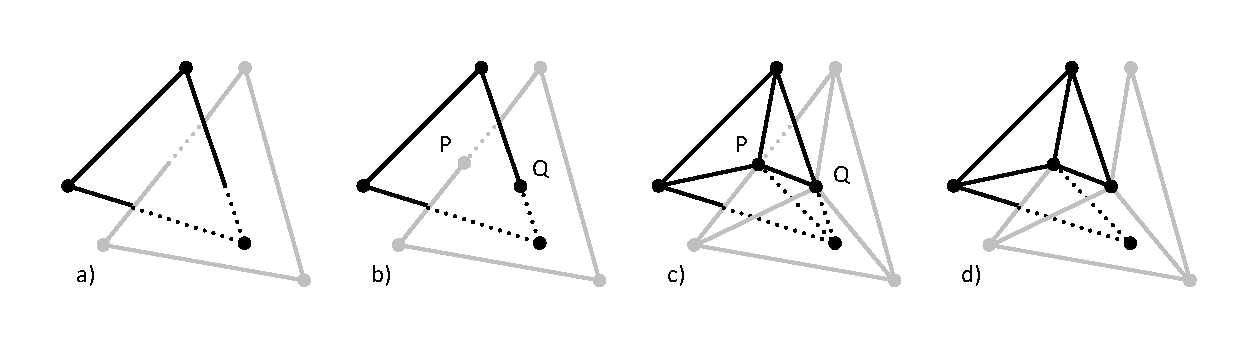
\includegraphics[width=1.0\textwidth]{pics/pic_algorithm_phases_s.pdf}
\captionstyle{center}\caption{Стадии устранения самопересечений.}\label{fig:pic_algorithm_phases_s}
\end{figure}

На рис.~\ref{fig:pic_algorithm_phases_s} представлены 4 фазы алгоритма устранения пересечений.
На первой фазе (рис.~\ref{fig:pic_algorithm_phases_s}, a) выполняется поиск всех пар ячеек (треугольников) которые потенциально пересекаются.
На второй фазе (рис.~\ref{fig:pic_algorithm_phases_s}, b) ищутся все точки пересечения треугольников (на данном рисунке показаны точки пересечения $P$ и $Q$).
На третьей фазе (рис.~\ref{fig:pic_algorithm_phases_s}, с) выполнятся разбиение пересекающихся треугольников на более мелкие таким образом, чтобы в получившейся измельченной сетке были только смежные по ребрам и вершинам треугольники (не было пересечений по внутренним точкам).
Очевидно, что после выполнения третьей фазы алгоритма в сетке могут образоваться ребра, инцидентные более чем двух ячейкам (на рис.~\ref{fig:pic_algorithm_phases_s}, с ребро $PQ$ инцидентно сразу четырем ячейкам).
Поэтому на четвертой фазе алгоритма (рис.~\ref{fig:pic_algorithm_phases_s}, d) осуществляется удаление лишних ячеек сетки (удаляются множества ячеек, которые образуют внутренние полости сетки).

Далее рассмотрим подробнее каждую из приведенных фаз алгоритма по-отдельности.

\section{Поиск пар потенциально пересекающихся треугольников}

Сначала для устранения самопересечений сетки необходимо найти все пары пересекающихся (но не смежных) треугольников.
Конечно к этому вопросу можно подойти напрямую, рассмотрев все $n$ треугольников из расчетной сетки и выполнив анализ на пересечение всех $\frac{1}{2}n(n - 1)$ пар.
Однако, такой подход займет большое количество времени, так как количество треугольников в расчетной сетке велико, а сама процедура определения пересечения двух треугольников нетривиальна.
Будем решать поставленную задачу по-другому.

Во-первых, вместо пар пересекающихся треугольников будем искать пары потенциально пересекающихся треугольников.
Для этого введем следующие понятия.
Для треугольника $ABC$ назовем его боксом прямоугольный параллелепипед $[min(A_x, B_x, C_x), max(A_x, B_x, C_x)] \times [min(A_y, B_y, C_y), max(A_y, B_y, C_y)] \times [min(A_z, B_z, C_z), max(A_z, B_z, C_z)]$.
Будем говорить, что два треугольника потенциально пересекаются, если пересекаются их боксы.
В отличие от пересечения треугольников, определение пересечения прямоугольных параллелепипедов (со сторонами, параллельными осям координат) это простая операция.
По аналогии с боксом треугольника можно определить бокс произвольной геометрической фигуры, а также множества таких геометрических фигур.
Мы будем использовать бокс множества треугольников.

Построим вспомогательный объект, называемый облаком треугольников.
В данное облако включим все треугольники расчетной сетки.
В качестве дополнительного поля данных облака треугольников будем использовать его бокс.
Теперь разделим облако треугольников на два подоблака с помощью сечения произвольной плоскостью (на рис.~\ref{fig:pic_triangles_cloud_s} показан двумерная иллюстрация данного процесса).
Каждый треугольник исходного облака отнесем в то подоблако, которое соответствует той части полупространства, в которую попал центр треугольника.
Таким образом, для рассматриваемого облака треугольников образованы два дочерних подоблака.
Заметим, что делить подоблако не обязательно ровно на два дочерних подоблака, число дочерних подоблаков может быть произвольным.
Продолжая процесс деления облаков треугольников далее, получим структуру, называемую деревом облаков, в корне которого находится все множество треугольников, а в листах -- отдельные треугольники.

\begin{figure}[h]
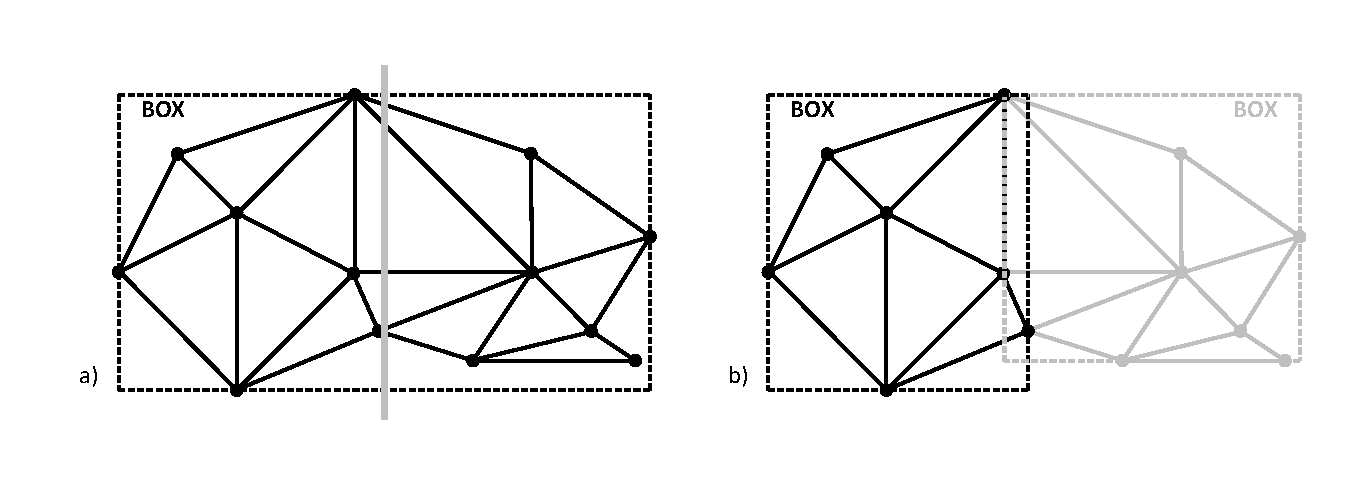
\includegraphics[width=1.0\textwidth]{pics/pic_triangles_cloud_s.pdf}
\captionstyle{center}\caption{Формирование облака треугольников.}\label{fig:pic_triangles_cloud_s}
\end{figure}

С помощью образованного вспомогательного дерева облаков треугольников можно быстро находить потенциально пересекающиеся треугольники.
Для этого достаточно воспользоваться следующим фактом: если два облака треугольников $T_1$ и $T_2$ не являются потенциально пересекающимися (то есть их боксы не пересекаются), то любые два треугольника $t_1 \in T_1$ и $t_2 \in T_2$ не являются потенциально пересекающимися.
При используя древовидного поиска потенциально пересекающихся треугольников с помощью вложенных боксов облаков треугольников время перебора всех треугольников в множестве меняется с линейного на логарифмическое, что сильно ускоряет расчеты.

\section{Поиск точек пересечения треугольников}

После того, как определены все пары потенциально пересекающихся треугольников, необходимо определить точки их пересечения.
Отметим следующий факт: если два треугольника пересекаются в пространстве, то обязательно хотя бы одна сторона одного треугольника должна пересекать другой треугольник.
Другими словами, все точки пересечения двух треугольников не могут быть одновременно внутренними точками одного треугольника и внутренними точками второго треугольника.
Поэтому задача поиска пересечений двух треугольников сводится к задаче пересечения одного треугольника со сторонами второго (и наоборот).

Исходя из этого простого факта, для определения всех точек пересечения треугольников достаточно решить следующие частные задачи: установление факта совпадения двух вершин (рис.~\ref{fig:pic_intersection_s}, a), установление факта попадания точки на отрезок (рис.~\ref{fig:pic_intersection_s}, b), установление пересечения двух отрезков в пространстве (рис.~\ref{fig:pic_intersection_s}, c), установление факта пересечения отрезка с треугольником (рис.~\ref{fig:pic_intersection_s}, d). 

\begin{figure}[h]
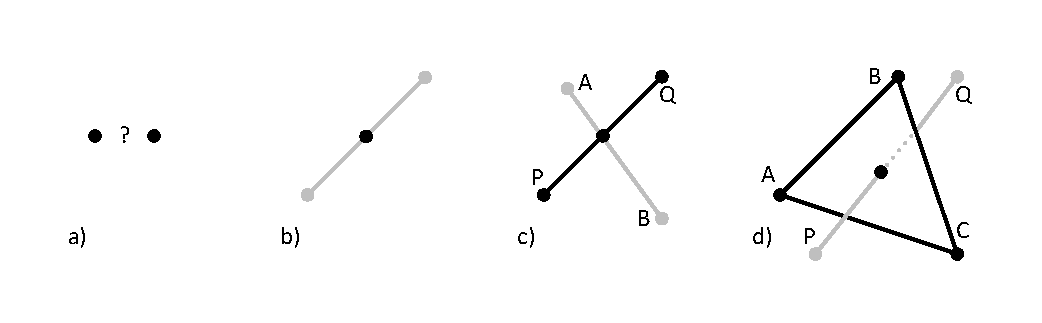
\includegraphics[width=1.0\textwidth]{pics/pic_intersection_s.pdf}
\captionstyle{center}\caption{Поиск точек пересечения разных геометрических примитивов.}\label{fig:pic_intersection_s}
\end{figure}

Из приведенных частных задач внимания заслуживают только две последние.
Для их решения будем использовать представление геометрических объектов в виде геометрического места точек, а именно: отрезок $PQ$ в пространстве будем представлять в виде геометрического места точек $P + \phi(Q - P), 0 \le \phi \le 1$, а треугольник $ABC$ в пространстве будем записывать в виде $A + \alpha(B - A) + \beta(C - A), \alpha \ge 0, \beta \ge 0, \alpha + \beta \le 1$ (данные записи понимаются в векторном виде).

Тогда для поиска пересечений двух отрезков $AB$ и $PQ$ в пространстве достаточно решить следующую систему:

\begin{equation}
\begin{cases}
A_x + \psi(B_x - A_x) = P_x + \phi(Q_x - P_x) \\
A_y + \psi(B_y - A_y) = P_y + \phi(Q_y - P_y) \\
A_z + \psi(B_z - A_z) = P_z + \phi(Q_z - P_z) \\
0 \le \psi \le 1 \\
0 \le \phi \le 1
\end{cases}
\end{equation}

У данной системы может не быть решений, быть ровно одно решение и быть бесконечно много решений.
Внимания заслуживает случай бесконечного количества решений.
В этом случае мы имеем дело с наложением двух отрезков друг на друга, и задача поиска пересечений сводится к задачам определения совпадения двух точек и определения попадания точки на отрезок.

Для поиска пересечений треугольника $ABC$ с отрезком $PQ$ необходимо решить следующую систему уравнений:

\begin{equation}
\begin{cases}
A_x + \alpha(B_x - A_x) + \beta(C_x - A_x) = P_x + \phi(Q_x - P_x) \\
A_y + \alpha(B_y - A_y) + \beta(C_y - A_y) = P_y + \phi(Q_y - P_y) \\
A_z + \alpha(B_z - A_z) + \beta(C_z - A_z) = P_z + \phi(Q_z - P_z) \\
\alpha \ge 0 \\
\beta \ge 0 \\
\alpha + \beta \le 1 \\
0 \le \phi \le 1
\end{cases}
\end{equation}

Данная система может не иметь решений, иметь ровно одно решение и иметь бесконечное количество решений.
В данном случае также особой обработки требует ситуация бесконечного количества решений, в которой задача сводится к определению точек пересечения двух отрезков.

После выполнения поиска пересечений всех геометрических объектов необходимо поместить найденные точки пересечения на ребра расчетной сетки (если пересечение произошло по ребру), либо в ячейки (если пересечение произошло по внутренной точке треугольника).
После чего выполняется переход к следующей фазе алгоритма.

\section{Разбиение треугольников на более мелкие}

После выполнения предыдущей фазы алгоритма на некоторое элементы расчетной сетки (ребра и треугольники) были нанесены точки самопересечения.
На данной фазе алгоритма необходимо таким образом измельчить сетку, чтобы все такие нанесенные точки стали узлами новой сетки.
Это наиболее простая процедура из всех шагов алгоритма.
Если некоторая нанесенная точка $P$ попала внутрь треугольника $ABC$ (рис.~\ref{fig:pic_split_s}, a) то достаточно сделать разбиение $ABC \rightarrow ABP, BCP, ACP$ (рис.~\ref{fig:pic_split_s}, b).
В случае попадания сразу нельскольких точек внутрь треугольника разбиение выполняется рекурсивно.
Если некоторая нанесенная точка $P$ попала на некоторое ребро $AC$ треугольника $ABC$ (рис.~\ref{fig:pic_split_s}, c), то необходимо выполнить разбиение $ABC \rightarrow ABP, CBP$.
При этом, если ребро $AC$ не является границой расчетной сетки, то оно инцидентно еще одному треугольнику, который также должен быть разбит по этой точке $P$ (рис.~\ref{fig:pic_split_s}, d).

\begin{figure}[h]
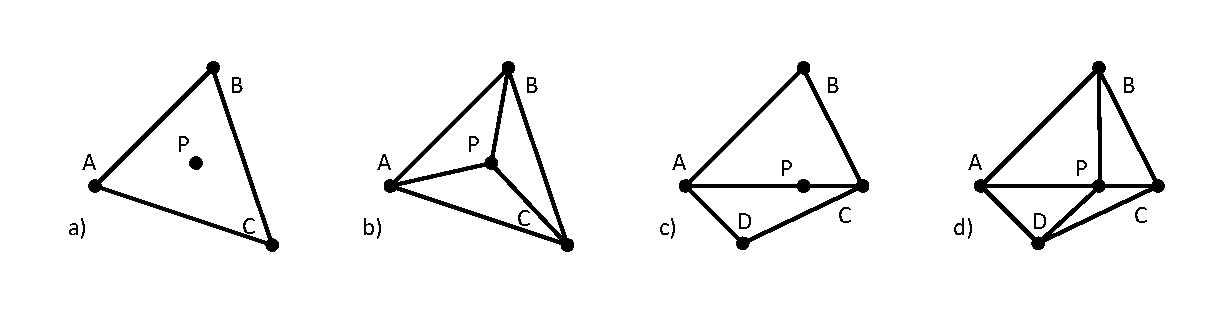
\includegraphics[width=1.0\textwidth]{pics/pic_split_s.pdf}
\captionstyle{center}\caption{Разбиение треугольников по точкам пересечения.}\label{fig:pic_split_s}
\end{figure}

Следует отметить, что при таком подходе могут появляться треугольники с углами, близкими к нулевым.
Для того, чтобы качество сеток сильно не понижалось от таких треугольников следует избавляться.
Например, если точка $P$ внутри треугольника $ABC$ окажется слишком близко к стороне $AC$ (рис.~\ref{fig:pic_split_s}, a), то угол $\angle APC$ окажется близок к развернутому, и в этом случае для сохранения качества сетки целесообразно переместить точку $P$ на сторону $AC$.

\section{Удаление лишних ячеек}

Последним шагом алгоритма является удаление лишних ячеек после измельчения сетки.
В местах самопересения сетки после ее измельчения образуются ребра, которые могут быть инцидентны более чем двум ячейкам (в классическом случае это 4 ячейки, как показано на рис.~\ref{fig:pic_del_extra_s}).
При этом для корректного представления поверхности требуется, чтобы данное ребро было инцидентно только двум ячейкам (остальные ячейки относятся к скрытой области самопересечения и описывают полость, которая должна быть вырезана).

\begin{figure}[h]
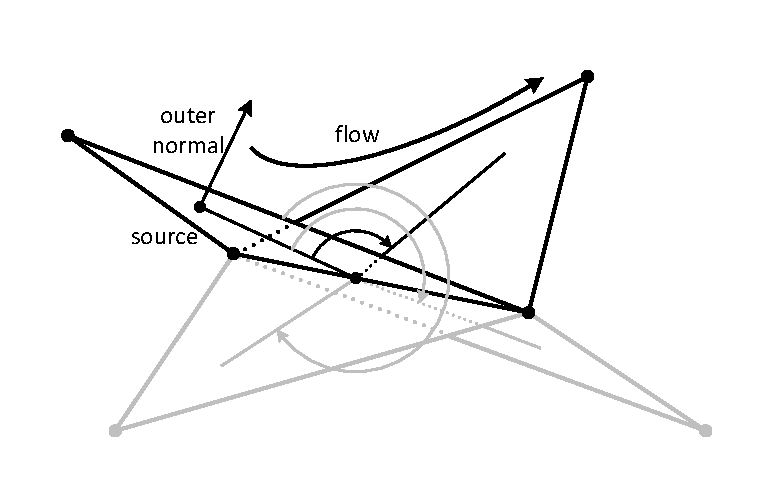
\includegraphics[width=0.7\textwidth]{pics/pic_del_extra_s.pdf}
\captionstyle{center}\caption{Удаление лишних ячеек.}\label{fig:pic_del_extra_s}
\end{figure}

Для определения лишних ячеек необходимо уметь идентифицировать хотя бы одну ячейку, которая точно относится к поверхности (на рис.~\ref{fig:pic_del_extra_s} для такой ячейки обозначена внешняя нормаль).
Этого можно достичь путем обхода поверхности из области, где точно отсутствуют самопересечения.
То есть, если известно, что какая-то ячейка расчетной сетки точно относится к поверхности и одна имеет ровно одну смежную ячейку по некоторому ребру, то эта смежная ячейка также относится к поверхности (однозначно определяется с какой на какую ячейку осуществляется перетекание потока).
Выполняя обход таким образом рано или поздно мы либо обойдем все ячейки (тогда самопересечений нет и сетку корректировать не надо), либо придем к ребру через которое нельзя однозначно определить перетекание потока (как показана на рис.\ref{fig:pic_del_extra_s}).
Для таких ребер будем поступать следующим образом.
Ячейку, про которую точно известна ее принадлежность поверхности, будем называть "хорошей".
В качестве второго претендента на принадлежность к поверхности выберем ту ячейку, для которой угол поворота хорошей ячейки в направлении внешней нормали хорошей ячейки до совпадения будем минимальным.

\section{Заключение}

\begin{figure}[h]
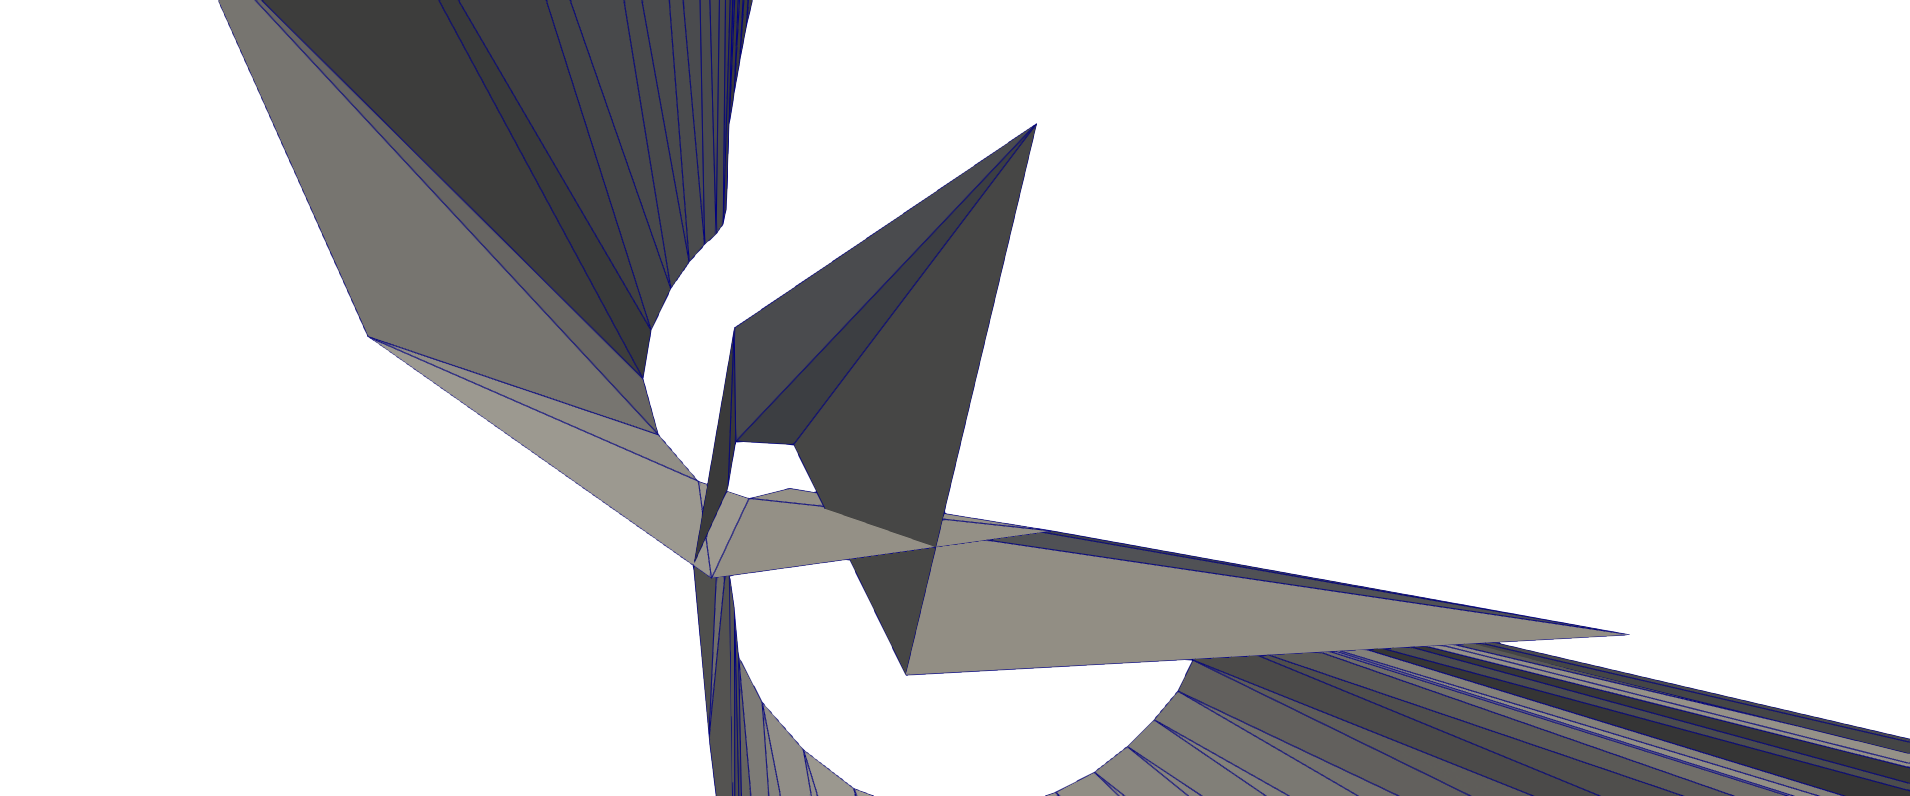
\includegraphics[width=1.0\textwidth]{pics/pic_example_before.png}
\captionstyle{center}\caption{Пример расчетной сетки с самопересечением.}\label{fig:pic_example_before}
\end{figure}

\begin{figure}[h]
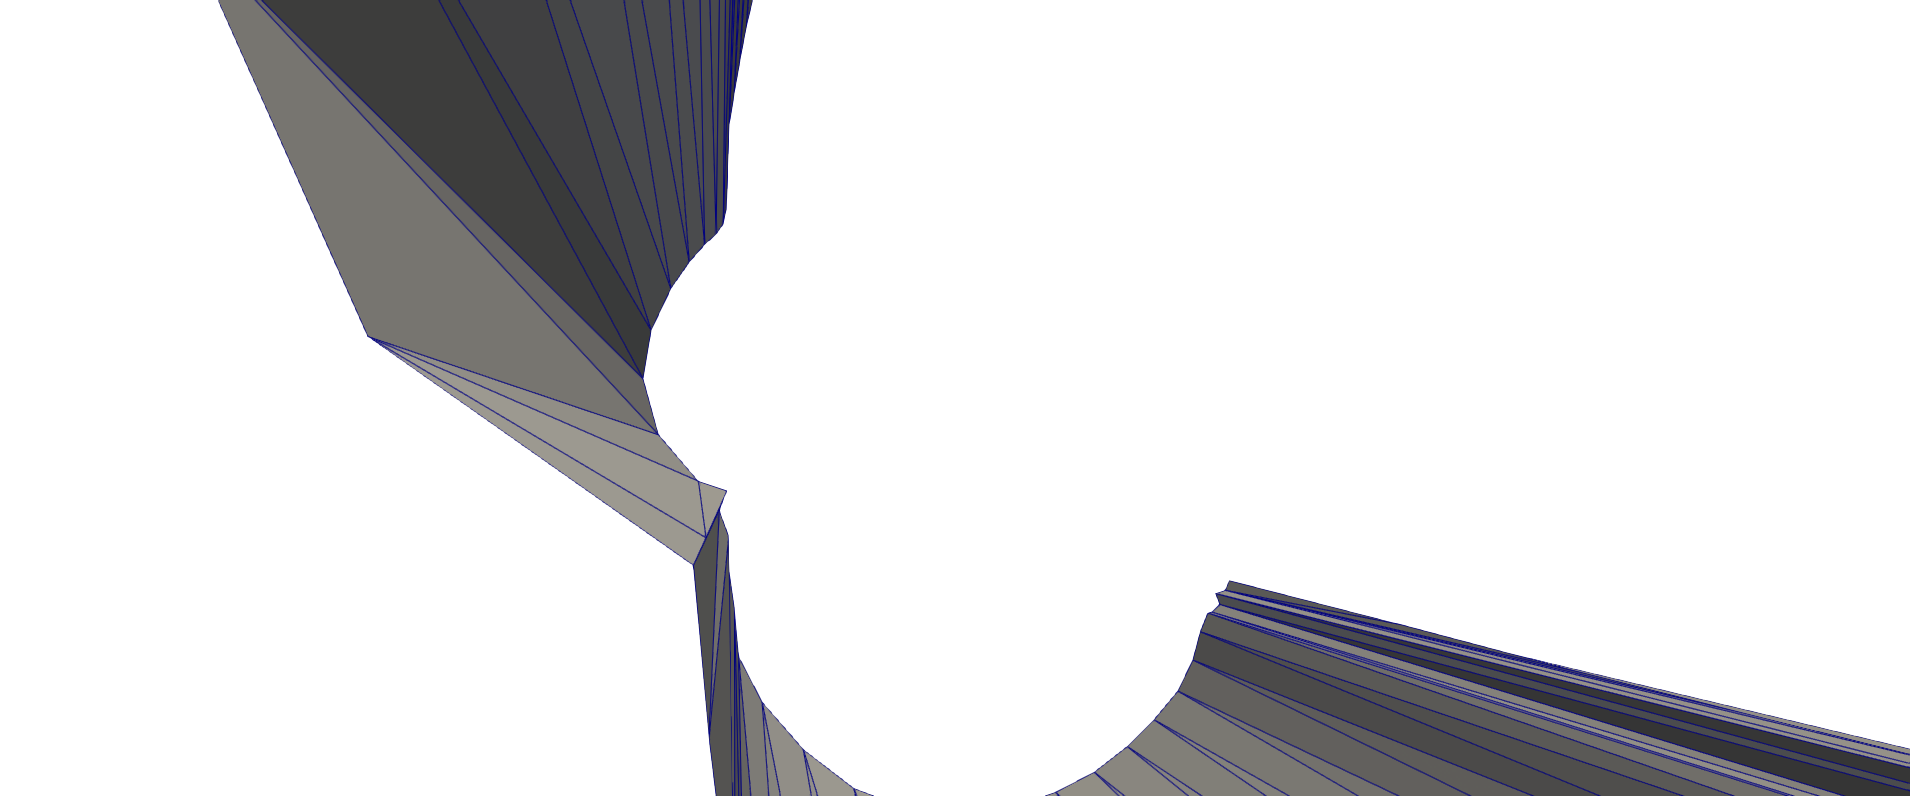
\includegraphics[width=1.0\textwidth]{pics/pic_example_after.png}
\captionstyle{center}\caption{Результата устранения самопересечения.}\label{fig:pic_example_after}
\end{figure}

\begin{acknowledgments}
TODO
\end{acknowledgments}

\begin{thebibliography}{99}

% ice accretion task

\bibitem{Myers}
\refitem{article}
T.~Myers, \textquotedblleft Extension to the Messinger model for aircraft icing,\textquotedblright \ AIAA J. \textbf{39}, 211--218 (2001).

\bibitem{Farzaneh}
\refitem{article}
P.~Farzaneh and G.~Bouchard, \textquotedblleft Modeling a water flow on an icing surface,\textquotedblright \ in \textit{Proceedings of the International Workshop on Atmospheric Icing of Structures IWAIS XI, Montr\'eal, 2005}.

\bibitem{Dong}
\refitem{article}
W.~Dong, J.~Zhu, and X.~Min, \textquotedblleft Calculation of the heat transfer and temperature on the aircraft anti-icing surface,\textquotedblleft \ in \textit{Proceedings of the 27th International Congress of the Aeronautical Sciences, 2010}.

\bibitem{Beaugendre}
\refitem{misc}
H.~Beaugendre, \textquotedblleft A PDE-based approach to in-flight ice accretion,\textquotedblright \ PhD Thesis (Dep. of Mech. Eng., McGill Univ., Montr\'eal, Qu\'ebec, 2003).

% ice accretion software

\bibitem{Bourgault}
\refitem{article}
Y.~Bourgault, H.~Beaugendre, and W.~Habashi, \textquotedblleft Development of a shallow-water icing model in FENSAP-ICE,\textquotedblright \ J. Aircraft \textbf{37}, 640--646 (2000).

\bibitem{Wright}
\refitem{article}
W.~Wright, P.~Struck, T.~Bartkus, and G.~Addy, \textquotedblleft Recent advances in the LEWICE icing model,\textquotedblright \ SAE Int. Technical Paper (2015).

\bibitem{Beld}
\refitem{misc}
E.~Beld, \textquotedblleft Droplet impingement and film layer modeling as a basis for aircraft icing simulations in OpenFOAM,\textquotedblright \ Internship Report (Eng. Fluid Dynamics Department, Univ. Twente, 2013).

\bibitem{Domingos}
\refitem{article}
R.~Domingos and S.~Silva, \textquotedblleft 3D computational methodology for bleed air ice protection system parametric analysis,\textquotedblright \ SAE Int. technical paper (2015).

\bibitem{Aksenov}
\refitem{article}
A.~A.~Aksenov, P.~M.~Byvaltsev, S.~V.~Zhluktov, K.~E.~Sorokin, A.~A.~Babulin, and V.~I.~Shevyakov, \textquotedblleft Numerical simulation of ice accretion on airplane surface,\textquotedblright \ in \textit{Proceedings of AIP Conference, 2019}.

% remeshing

\bibitem{BourgaultCote}
\refitem{article}
S.~Bourgault-C\^ot\'e, K.~Hasanzadeh, P.~Lavoie, and E.~Laurendeau, \textquotedblleft Multi-layer icing methodologies for conservative ice growth,\textquotedblright \ in \textit{Proceedings of 7th European Conference for Aeronautics and Aerospace Sciences EUCASS, 2017}.

\bibitem{Fortin}
\refitem{article}
G.~Fortin, A.~Ilinca, J.-L.~Laforte, and V.~Brandi, \textquotedblleft New roughness computation method and geometric accretion model for airfoil icing,\textquotedblright \ J. Aircraft \textbf{41}, 119--1127 (2004).

\bibitem{Thompson}
\refitem{article}
D.~Thompson, X.~Tong, Q.~Arnoldus, E.~Collins, D.~McLaurin, and E.~Luke, \textquotedblleft Discrete surface evolution and mesh deformation for aircraft icing applications,\textquotedblright \ in \textit{Proceedings of 5th AIAA Atmospheric and Space Environments Conference, 2013}.

\bibitem{Tong}
\refitem{article}
X.~Tong, D.~Thompson, Q.~Arnoldus, E.~Collins, and E.~Luke, \textquotedblleft Three-dimensional surface evolution and mesh deformation for aircraft icing applications,\textquotedblright \ J. Aircraft \textbf{54}, 1--17 (2016).

% self-intersections elimination

\bibitem{Charton}
\refitem{article}
J.~Charton, S.~Baek, and Y.~Kim, \textquotedblleft Mesh repairing using topology graphs,\textquotedblright \ J. of Computational Design and Engineering \textbf{8}, 251--267 (2021).

\bibitem{Jung}
\refitem{article}
W.~Jung, H.~Shin, and B.~K.~Choi, \textquotedblleft Self-intersection removal in triangular mesh offsettings,\textquotedblright \ CAD J. \textbf{1}, 477--484 (2004).

\bibitem{Skorkovska}
\refitem{article}
V.~Skorkovsk\'a, I.~Kolingerov\'a, and B.~Benes, \textquotedblleft A simple and robust approach to computation of meshes intersection,\textquotedblright \ in \textit{Proceedings of the 13th International Joint Conference on Computer Vision, Imaging and Computer Graphics Theory and Applications VISIGRAPP, 2018}.

\end{thebibliography}

\end{document}
